\documentclass{ceurart}


\begin{document}

%%
%% Rights management information.
%% CC-BY is default license.
\copyrightyear{2023}
\copyrightclause{Copyright for this paper by its authors.\\
  Use permitted under Creative Commons License Attribution 4.0
  International (CC BY 4.0).}

%%
%% This command is for the conference information
\conference{CLEF 2023: Conference and Labs of the Evaluation Forum, September 18--21, 2023, Thessaloniki, Greece}

%%
%% The "title" command
\title{Your Title in Title Case}

\title[mode=sub]{Notebook for the iDPP Lab on Intelligent Disease Progression Prediction at CLEF 2023}

%%
%% The "author" command and its associated commands are used to define
%% the authors and their affiliations.
\author[1]{Name SurnameA}[%
orcid=0000-0000-0000-0001,
email=name.surnameA@email.org,
url=http://www.name.surnameA.org/,
]

\author[1,2]{Name SurnameB}[%
orcid=0000-0000-0000-0002,
email=name.surnameB@email.org,
url=http://www.name.surnameB.org/,
]

\author[3]{Name SurnameC}[%
orcid=0000-0000-0000-0003,
email=name.surnameC@email.org,
url=http://www.name.surnameC.org/,
]

\address[1]{Organization 1, Somewhere}
\address[2]{Organization 2, Somewhere}
\address[3]{Organization, 3 Somewhere}


%%
%% The abstract is a short summary of the work to be presented in the
%% article.
\begin{abstract}
  A clear and well-documented \LaTeX{} document is presented as an
  article formatted for publication by CEUR-WS in a conference
  proceedings. Based on the ``ceurart'' document class, this article
  presents and explains many of the common variations, as well as many
  of the formatting elements an author may use in the preparation of
  the documentation of their work.
\end{abstract}

%%
%% Keywords. The author(s) should pick words that accurately describe
%% the work being presented. Separate the keywords with commas.
\begin{keywords}
  keyword 1 \sep
  keyword 2 \sep
  keyword 3 
\end{keywords}

%%
%% This command processes the author and affiliation and title
%% information and builds the first part of the formatted document.
\maketitle


\section{Introduction}
\label{sec:introduction}

Introduce the context, motivations, and goals of your project.

The paper is organized as follows: Section~\ref{sec:related} introduces related works; Section~\ref{sec:methodology} describes our approach; Section~\ref{sec:setup} explains our experimental setup; Section~\ref{sec:results} discusses our main findings; finally, Section~\ref{sec:conclusion} draws some conclusions and outlooks for future work.

\section{Related Work}
\label{sec:related}

Describe related works, i.e. previous approaches to solve your problem you have started or improved from.

\section{Methodology}
\label{sec:methodology}

Describe the methodology you have adopted, the features you have used for prediction, the architecture of your system, your workflow, etc.

\section{Experimental Setup}
\label{sec:setup}

Describe the experimental setup, i.e.
\begin{itemize}
	\item url to git repository and its organization
	\item hardware used for experiments
	\item ...
\end{itemize}


For the detailed description of the datasets and the evaluation measures, you can cite the overview paper which will provided you by organizer and avoid duplicating content.

\section{Results}
\label{sec:results}

Provide a summary of the performance on the CLEF 2022 dataset.

Conduct a statistical validation of the experimental results.

Discuss the results and any relevant issues.

\section{Conclusions and Future Work}
\label{sec:conclusion}

Provide a summary of what are the main achievements and findings. 

Discuss future work, e.g. what you may try next and/or how your approach could be further developed.


\section{Misc [TO BE REMOVED]}


\subsection{Figures}

Put the caption under the figure. Example of reference to Figure~\ref{fig:sample-figure}.

\begin{figure}
  \centering
  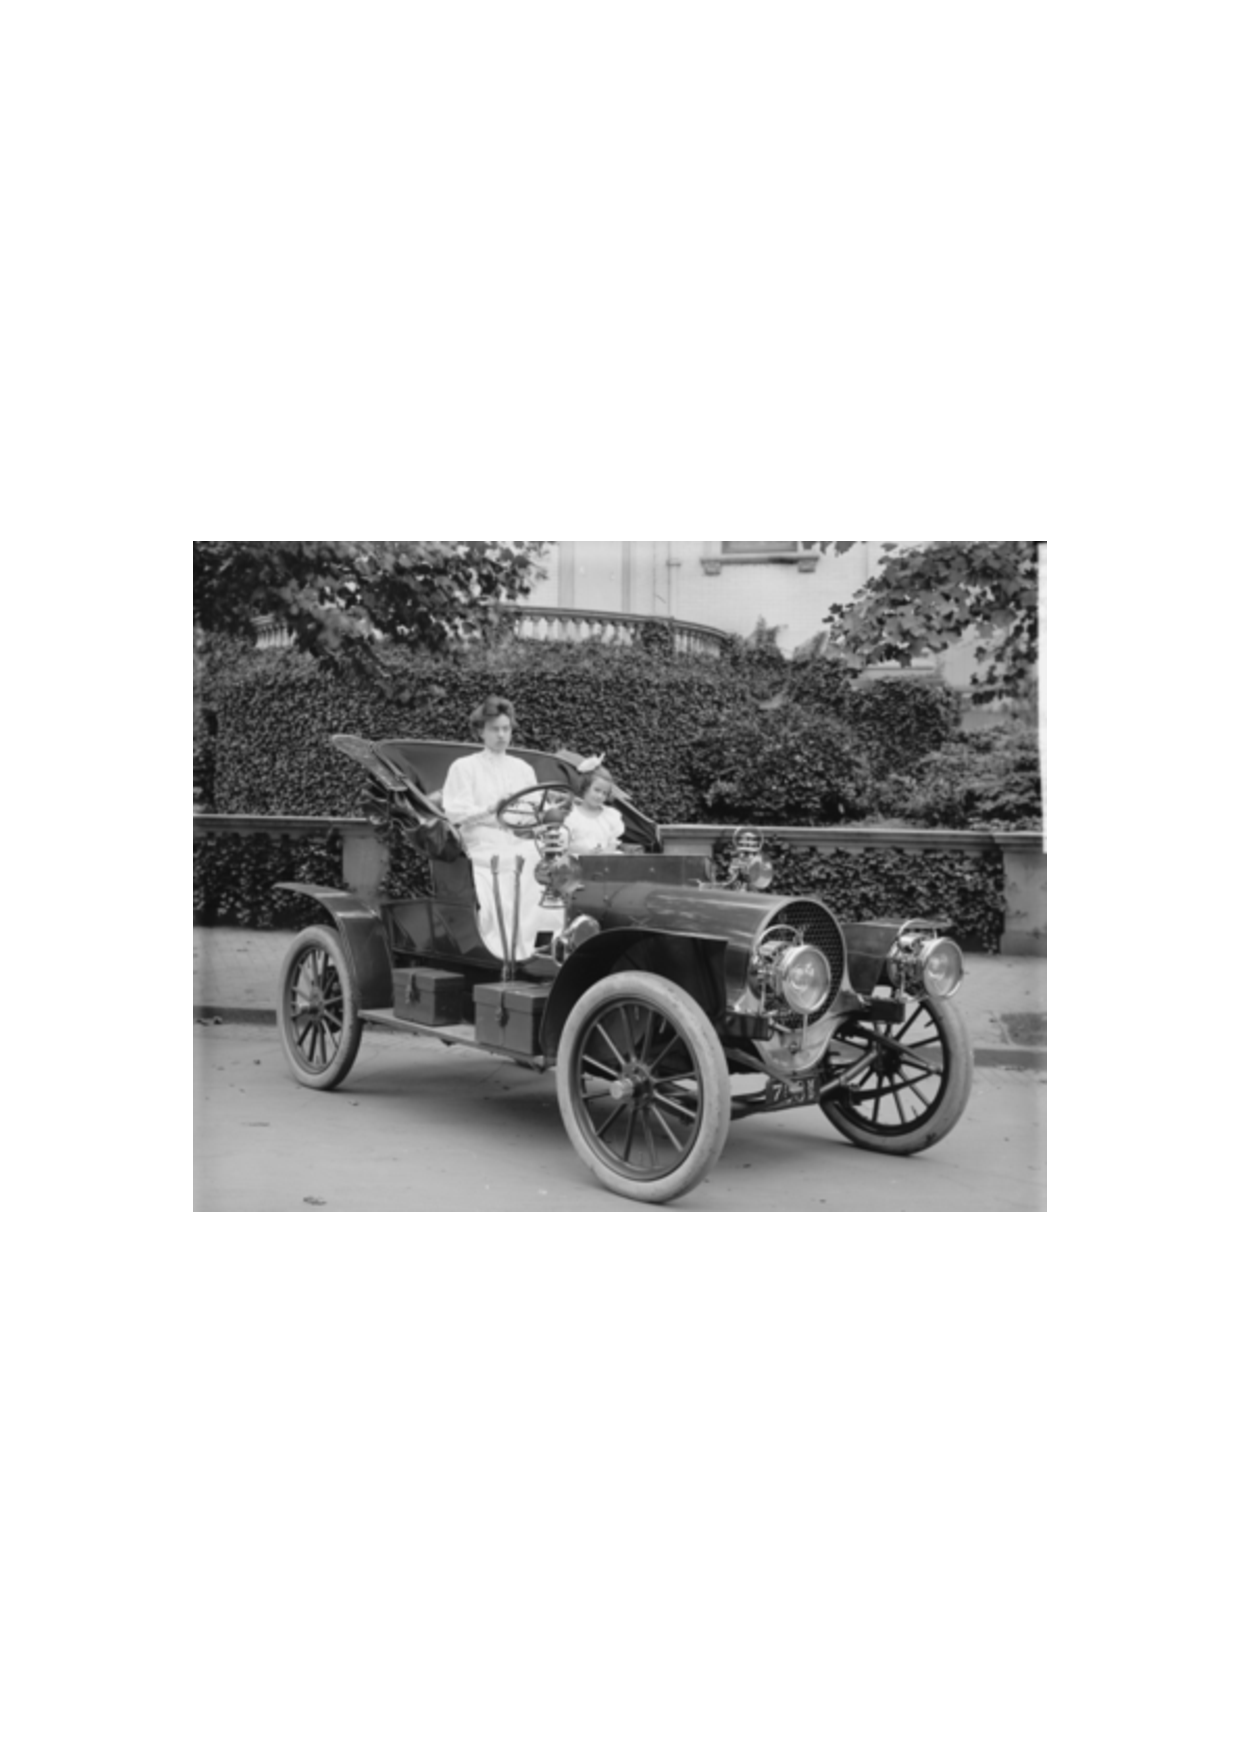
\includegraphics[width=0.8\linewidth]{figure/sample.pdf}
  \caption{1907 Franklin Model D roadster. Photograph by Harris \& Ewing, Inc. [Public domain], via Wikimedia Commons. (\url{https://goo.gl/VLCRBB}).}
  \label{fig:sample-figure}
\end{figure}

\subsection{Tables}

Put the caption above the table. Example of reference to Table~\ref{tab:sample-table}.

\begin{table}
  \caption{Frequency of Special Characters}
  \label{tab:sample-table}
  \centering
  \begin{tabular}{|c|c|l|}
    \toprule
    Non-English or Math&Frequency&Comments\\
    \midrule
    \O & 1 in 1,000& For Swedish names\\
    $\pi$ & 1 in 5& Common in math\\
    \$ & 4 in 5 & Used in business\\
    $\Psi^2_1$ & 1 in 40,000& Unexplained usage\\
  \bottomrule
\end{tabular}
\end{table}

See the \texttt{booktab} packaged documentation for further options.

\subsection{Bibliography}

Example of citations:
\begin{itemize}
	\item name: \citet{Turing1936}
	\item parenthesis: \citep{Turing1936}
\end{itemize}

See the \texttt{natbib} packaged documentation for further options.


%% Define the bibliography file to be used
\bibliography{bibliography}


\end{document}
